\documentclass{../fal_assignment}
\graphicspath{ {../} }

\usepackage{enumitem}
\setlist{nosep} % Make enumerate / itemize lists more closely spaced
\usepackage[T1]{fontenc} % http://tex.stackexchange.com/a/17858
\usepackage{url}
\usepackage{todonotes}

\title{Continuing Personal Development (CPD) Tasks --- Semester Two}
\author{Dr Michael Scott}
\module{COMP240}

\begin{document}

\maketitle
%\begin{marginquote}
%    ``Students come into programming classes with a broad range of backgrounds ---
%    some have experience in several programming languages, others have never programmed before in their life.
%    
%    Being able to engage with the community and support each other is important.
%    Upload your code to GitHub and receive feedback from experienced peers.
%    Review your peers' work yourself and really consider what `quality' actually means
%    and what `good' source code looks like.
%    Debate, argue, and question others about it ---
%    an open and sustained discourse is an excellent way to learn ---
%    for both beginners and adepts!''
%\end{marginquote}
\begin{marginquote}
    ``Remember, learning to program can take a surprising amount of time \& effort --- students may get there at different rates, but all students who put in the time \& effort get there eventually. Making good use of [reflection and deliberate practice] are an essential part of this process.''
    
    --- Professor Quintin Cutts

    \marginquoterule

    ``Continuing [Personal] Development is the responsibility of individuals for systemic maintenance, development and broadening of knowledge, skills and attitudes, to ensure continuing competence as a professional, throughout their careers .''
    
    --- International Pharmaceutical Federation
\end{marginquote}

\marginpicture{flavour_pic}{
    \textit{Event[0]}, a student project, was commercially released three years after graduation. Diligence and persistence are key.
}
\section*{Introduction}

In this assignment, you critically reflect on your progress across the Semester. This involves reviewing key weaknesses that influence the quality of your work. From this, you develop plans of continuing personal development.

Such reflection and planning is an extremely important part of learning games development. Research shows that deliberate practice is very effective at nurturing expertise in software engineering. Everyone properly adopting CPD eventually succeeds, despite the challenging nature of programming.

This assignment is formed of several parts:

\begin{enumerate}[label=(\Alph*)]
    \item \textbf{Write} a series of brief weekly reports (about 100-200 words) that will:
    	\begin{enumerate}[label=\roman*.]
    		\item \textbf{describe} your progress;
    		\item \textbf{identify} and \textbf{assess} at least \textbf{one} challenge you have encountered;
    		\item and then \textbf{outline} at least \textbf{one} specific action that will help you to overcome this challenge.
	\end{enumerate}
	    \item \textbf{Write}, in addition to your weekly reports, a brief summary of your experience (about 100-200 words) that will:
    	\begin{enumerate}[label=\roman*.]
    		\item \textbf{specify} your career goals;
    		\item \textbf{describe} your progress towards these goals;
    		\item \textbf{identify} at least \textbf{five} key challenges across different domains;
    		\item and then \textbf{outline five} SMART actions that may help you to overcome these challenges.
	\end{enumerate}
    \item \textbf{Write} a draft 1200-word report that must:
    	\begin{enumerate}[label=\roman*.]
    		\item \textbf{identify five} key skills that you consider obstacles;
    		\item \textbf{justify} the relevance \textbf{and} importance of \textbf{each} of these skills, with respect to professional game development;
    		\item \textbf{assess} your application of \textbf{each} of these skills, \textit{describing how} they affected the quality of your work;
    		\item and then \textbf{suggest how} to overcome \textbf{each} of these obstacles, with reference to SMART actions.
	\end{enumerate}
    \item \textbf{Write} a final 1200-word report that must:
    	\begin{enumerate}[label=\roman*.]
    		\item \textbf{revise} any issues raised by your tutor or your peers.
	\end{enumerate}
\end{enumerate}

\subsection*{Assignment Setup}

This assignment is a \textbf{reflective writing task} and so regular reflection is expected. Fork the GitHub repository at the following URL:

\indent \url{https://github.com/Falmouth-Games-Academy/comp150-cpd}

Use the existing directory structure and, as required, extend this structure with sub-directories. Ensure that you maintain the \texttt{readme.md} file. 

Modify the \texttt{.gitignore} to the defaults for \textbf{TeX}. Please, also ensure that you add editor-specific files and folders to \texttt{.gitignore}. 

\subsection*{Part A}

Part A consists of a \textbf{multiple formative submissions}. This work is \textbf{individual} and will be assessed on a \textbf{threshold} basis. The following criteria are used to determine a pass or fail:

\begin{enumerate}[label=(\alph*)]
	\item Progress has been described with adequate detail;
	\item Problems and issues have been clearly explained and assessed;
	\item There is evidence of reflection;
	\item At least one appropriate SMART objective has been actioned;
\end{enumerate}

To complete Part A, write each report in the \texttt{readme.md} document. Separate each week with a heading. Attend the scheduled catch-up tutorials and show the document to your tutor. 

You will receive immediate \textbf{informal feedback} from your tutor.

\subsection*{Part B}

Part B is a \textbf{single formative submission}. This work is \textbf{individual} and will be assessed on a \textbf{threshold} basis. The following criteria are used to determine a pass or fail:

\begin{enumerate}[label=(\alph*)]
	\item Submission is timely;
	\item Enough work is available to conduct a meaningful review;
	\item A broadly appropriate review of a peer's work is submitted.
\end{enumerate}

To complete Part B, write each report in the \texttt{readme.md} document. Separate each week with a heading. Ensure that your summary is included at the top of the\texttt{readme.md} document under a separate heading. Then, attend the scheduled catch-up tutorials and show the document to your tutor. 

You will receive immediate \textbf{informal feedback} from your tutor.

\subsection*{Part C}

Part B is a \textbf{single formative submission}. This work is \textbf{individual} and will be assessed on a \textbf{threshold} basis. The following criteria are used to determine a pass or fail:

\begin{enumerate}[label=(\alph*)]
	\item Submission is timely;
	\item Enough work is available to conduct a meaningful review;
	\item A broadly appropriate review of a peer's work is submitted.
\end{enumerate}

To complete Part C, prepare a draft version of the CPD report. Use the rubric at the end of this document to inform the structure of the document. Ensure that the TeX source and compiled \texttt{*.pdf} are pushed to GitHub and a pull request is made prior to the scheduled task review session. Then, attend the scheduled CPD catch-up session.

You will receive immediate \textbf{informal feedback} from your tutor.

\subsection*{Part D}

Part D is a \textbf{single summative submission}. This work is \textbf{individual} and will be assessed on a \textbf{criterion-referenced} basis. Please refer to the assessment criteria in the marking rubric at the end of this document for further insight.

To complete Part D, revise the reflective report based on the feedback you have received. Then, upload the reflective report to the LearningSpace. Please note, the LearningSpace will only accept a single \texttt{*.pdf} file.

You will receive \textbf{formal feedback} three weeks after the final deadline.

\section*{Additional Guidance}

\textbf{Reflection} is taking time to examine thoughts, feelings, beliefs, values, attitudes and assumptions in the context of a specific topic, situation, problem, issue, or process. Part of reflection is relating these varied understandings to your experience, then analysing how and why something arose. Building upon this, you can predict future performance. \textbf{Planning}, therefore, is identifying which challenges can be overcome and setting a series of activities you do to resolve those challenges. \textbf{Learning} is engaging in those SMART actions, thereby improving your performance or at least fulfilling some pre-requisite to enhancing performance in the future. \textbf{Evaluating} is measuring your new level of performance. Use this to assess the quality of your actions. Not all actions will be successful . This is to be expected. Nevertheless, such evaluation will still need to feed-into your future reflection.

\begin{center}
    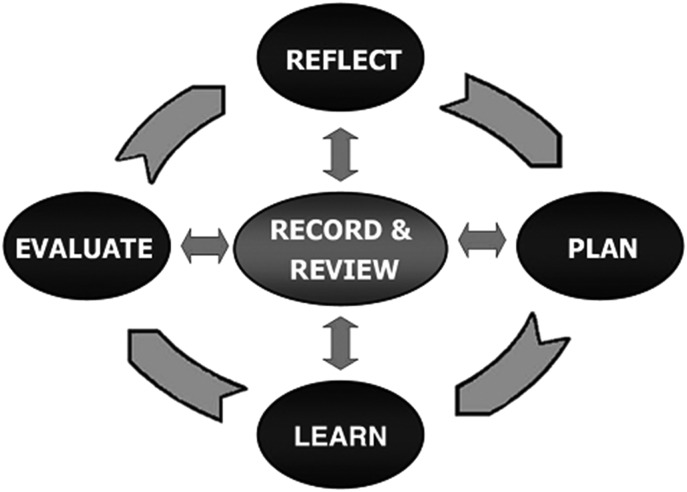
\includegraphics[scale=3]{ajpe798112-fig1} 
\end{center}

This process is cyclical, as illustrated above. It is, after all, \textit{continuous} personal development (also referred to as\textit{continuous professional development} by those in industry). You will be expected to engage in CPD throughout the degree course, with a deliverable every single semester. This will also form the cornerstone of ongoing improvement across the duration of your career.

A common mistake made by beginners to reflective writing is to merely describe the context and/or the experience. Avoid this. Description is not particularly important. It is the \textbf{analysis} and \textbf{evaluation} of an experience which is important. This is because it will reveal insights about yourself and your actions, which will help you to focus on the most relevant weaknesses.

Another common mistake is to focus too much on any one single domain. Your experience is holistic and there are many domains of practice that contribute to it. For example: the \textbf{affective domain}, such as your ability to identify and manage different mental states and emotions; the \textbf{interpersonal domain}, such as your ability to communicate and organise activity with peers; the \textbf{dispositional domain}, such as your ability to manage time and remain disciplined; the \textbf{cognitive domain}, such as your knowledge of programming languages or frameworks; and the \textbf{procedural domain}, such as your abilities to apply computing concepts and problem solving skills. 

Keep in mind that programming, in particular, is a skill that not only taxes groups of skills across all of these domains, but also demands a significant investment in time and energy to develop. It is a commitment! So, of course, regular practice is important. However! It is the \textbf{quality} of your practice that is more important than \textbf{quantity} of your practice.

Deliberate practice follows naturally from this continuous cycle of reflection, planning, practice, and evaluation. This means that \textbf{reflection is a forethought} rather than an afterthought. Avoid leaving reflection to the last minute. Focus on the ongoing development process early, and indeed, on the process itself. The quality of the end product may indicate the existence of challenges, but it is only through deep reflection on working practice that it becomes clear why those challenges arose and how to avoid them.

Effective deliberate practice is: conscious and intentional; designed with current skill in mind, forcing discomfort while avoiding frustration; provides relevant measures to track progress; and follows a repeatable structure.

When planning such practice, do not be too general. Consider \textbf{SMART} actions: \textbf{specific}; \textbf{measurable}; \textbf{achievable}; \textbf{relevant}; and \textbf{time-bound}. Ensure that your plan for future development meets all five of these criteria. Also note, problem solving and designing are particularly important programming skills and approaches to developing skills in these areas can be relevant.

When choosing which \textbf{skills} to focus on for this report, be specific. Avoid choosing broad skills that are clearly important for any student, such as ``time management'' or ``communication''. Instead, consider which \textbf{specific} aspects of these skills are a priority for \textbf{you}. We are not assessing your knowledge of general study skills, rather we are assessing your ability to analyse and reflect on your own learning as an individual.

\section*{FAQ}

\begin{itemize}
	\item 	\textbf{What is the deadline for this assignment?} \\ 
    		Falmouth University policy states that deadlines must only be specified on the MyFalmouth system.
    			    		    		
	\item 	\textbf{What should I do to seek help?} \\ 
    		You can email your tutor for informal clarifications. For informal feedback, make a pull request on GitHub. 
    		
    	\item 	\textbf{Is this a mistake?} \\ 	
    		If you have discovered an issue with the brief itself, the source files are available at: \\
    		\url{https://github.com/Falmouth-Games-Academy/bsc-assignment-briefs}.\\
    		 Please make a pull request and comment accordingly.
\end{itemize}

\section*{Additional Resources}

\begin{itemize}
    \item Ericsson, K.A., Krampe, R.T., and Tesch-Romer, C. (1993)The Role of Deliberate Practice in the Acquisition of Expert Performance. Psychological Review, 100(3), 363-406.
    \item Bolton, G.E.J. (2014) Reflective Practice: Writing and Professional Development. SAGE Publications: London.
\end{itemize}

\rubricyeartwo

\begin{markingrubric}
%
    \firstcriterion{Basic Competency Threshold}{40\%}
        \gradespan{1}{\fail At least one weekly report has not been submitted, is incomplete, or is unsatisfactory.}
        \gradespan{5}{All weekly reports, the CPD summary have been signed-off by your tutor at the relevant CPD catch-up session. The draft report was submitted for peer-review and a review was returned in-kind.}
%
    \criterion{Appropriateness, Specificity, and Relevance of Selection of Key Skills}{5\%}
%        \grade\fail 	Fewer than four appropriate key skills are mentioned.
        \grade \fail  	Fewer than five appropriate key skills are mentioned.
         \par 		Few skill domains have been considered.
        \grade 		Five appropriate key skills are mentioned.
        \par 		Most skill domains have been considered.
        \grade 		Five appropriate key skills are mentioned.
        \par 		All skill domains have been considered.
        \par 		At least two of the key skills are both specific and relevant.
        \grade 		Five appropriate key skills are mentioned.
        \par 		All skill domains have been considered.
        \par 		At least three of the key skills are both specific and relevant.
        \grade 		Five appropriate key skills are mentioned.
        \par 		All skill domains have been considered. There is little to no overlap.
        \par 		At least four of the key skills are both specific and a relevant.
        \par 		At least two of the key skills are a priority.
        \grade 		Five appropriate key skills are mentioned.
        \par 		All skill domains have been considered. There is little to no overlap.
        \par 		At least five of the key skills are both specific and a relevant.
        \par 		At least four of the key skills are a priority.
%
    \criterion{Adequacy of Self-Criticism in Relation to Key Skills}{10\%}
%        \grade\fail 	No self-criticism is made.
        \grade \fail  	Little to no self-criticism is made.
        \grade 		Some self-criticism.
           \par 		Little of the self-criticism is accurate.
        \grade 		Much self-criticism.
         \par 		Some of the self-criticism is accurate.
        \grade 		Considerable self-criticism.
         \par 		Much of the self-criticism is accurate.
        \grade 		Significant self-criticism.
         \par 		Nearly all of the self-criticism is accurate.
            \par 		Much of the self-criticism is pertinent.
        \grade 		Extensive self-criticism.
         \par 		Nearly all of the self-criticism is accurate.
            \par 		Nearly all of the self-criticism is pertinent.
%
    \criterion{Depth of the Reflection on the Application of Skills}{15\%}
 %       \grade\fail 	No reflection is evident.
        \grade \fail 	Little to no reflection is evident.
        \grade 		Some reflection is evident.
        \par 		Little depth of insight is demonstrated.
        \grade 		Much reflection is evident.
        \par 		Some depth of insight is demonstrated.
        \grade 		Considerable reflection is evident.
        \par 		Much depth of insight is demonstrated.
        \grade 		Significant reflection is evident.
        \par 		Significant depth of insight is demonstrated.
        \grade 		Extensive reflection is evident.
        \par 		Extensive depth of insight is demonstrated.
%
    \criterion{Appropriateness of Plan for Future Development}{15\%}
% \grade\fail 	No appropriate plans are proposed.
        \grade \fail	Less than five generally appropriate plans are proposed.
        \grade 		At least five generally appropriate plans are proposed. 
        \grade 		At least five specific and achievable plans are proposed. 
        \grade 		At least five specific and achievable plans are proposed. 
        \par 		At least three of the plans are also relevant.
        \grade 		At least five specific, relevant, and achievable plans are proposed. 
        \par 		At least three of the plans are also measurable and time-bound.
        \grade 		At least five specific, measurable, achievable, relevant, and time-bound plans are proposed. 
%
    \criterion{Mastery of Reflective Writing Style}{5\%}
        \grade\fail 	Little or no evidence of mastery for reflective writing.
         \par 		There is an accusatory and/or unconstructive tone.
        \grade 		Some evidence of mastery of reflective writing.
         \par 		The prose evokes a fair and constructive tone.
        \grade 		Much evidence of reflective writing.
         \par 		The prose evokes a balanced, critical, and constructive tone.
        \grade 		Considerable evidence of mastery of reflective writing.
         \par 		The prose evokes a balanced, critical, and constructive tone.
        \grade 		Significant evidence of mastery of reflective writing.
         \par 		The prose evokes a balanced, critical, and constructive tone.
        \grade 		Extensive evidence of mastery of reflective writing.
         \par 		The prose evokes a balanced, critical, and constructive tone.
%
    \criterion{Appropriateness of Spelling \& Grammar}{5\%}
%        \grade\fail 	Substantial spelling and/or grammar errors.
        \grade  \fail	Many spelling and/or grammar errors.
        \grade 		Some spelling and/or grammar errors.  
        \grade 		Few spelling and/or grammar errors.
        \grade 		Almost no spelling and/or grammar errors.
        \grade 		No spelling or grammar errors.
        \par 		Active voice is prevalent.
        \grade 		No spelling or grammar errors.
        \par 		Active voice is prevalent.
        \par 		Grammar is leveraged deliberately to draw attention to salient points.     
%
    \criterion{Appropriateness of Report Structure}{5\%}
%    \grade\fail 	There is no structure, or the structure is unclear.
        \grade \fail	There is little to no structure.
        \par 		Only a few sentences and paragraphs are well constructed.
        \grade 		There is some structure.
        \par 		Some sentences and paragraphs are well constructed.
        \grade 		There is much structure.
        \par 		Many sentences and paragraphs are well constructed.
        \par 		There is a clear introduction and conclusion.
        \grade 		There is considerable structure.
        \par 		Most sentences and paragraphs are well constructed.
        \par 		There is a clear and well-constructed introduction and conclusion.
        \grade 		There is significant structure, leveraged to effectively highlight the key takeaway points.
        \par 		Nearly all sentences and paragraphs are well constructed.
        \par 		There is a clear and well-constructed introduction and conclusion.
        \grade 		There is extensive structure, leveraged to effectively highlight the key takeaway points.
        \par 		All sentences and paragraphs are well constructed.
        \par 		There is a clear and well-constructed introduction and conclusion.
\end{markingrubric}

\end{document}